\documentclass{article}

\usepackage{geometry}
\usepackage{makecell}
\usepackage{array}
\usepackage{multicol}
\usepackage{setspace}
\usepackage{changepage}
\usepackage{booktabs}
\usepackage{titlesec}
\usepackage{graphicx}
\newcolumntype{?}{!{\vrule width 1pt}}
\renewcommand\theadalign{tl}
\setstretch{1.10}
\setlength{\parindent}{0pt}
\graphicspath{ {./images/} }

\titleformat{\section}
  {\normalfont\Large\bfseries}{\thesection}{1em}{}[{\titlerule[0.8pt]}]

\geometry{top=12mm, left=1cm, right=2cm}
\title{21W 520.302 Englisch: Kultur-Schwerpunktthemen III}
\author{Andreas Hofer}

\begin{document}
	\maketitle

	\section{Week 1 - Prelude - 07.10.2021}

	When talking about history one must always employ ciritcal thinking as history is often not a very objective matter. According to Neil de Grasse Tyson we are all born critical thinkers but are influenced by our parents and the school system, as inquisitiveness within a society is generally only permitted to a certain degree. \\
	\subsection{Hic sunt Dracones}
	In \textbf{The Demon-Haunted World} Carl Sagan tries explaining the scientific method and critical and skeptical thinking to a layman. In one chapter he talks about the \textbf{Dragon in the Garage"}, which is a dragon in my garage but you cannot see it, it also flies, is also incorporeal and breathes heatless flames so you cannot prove its existence. But if these dragons were to suddenly appear in many people's garages, is it more likely that they exist, despite there still not being any proof of their existence? My guess was, that this was an allegory about religion but it works for all unsourced claims. If you believe others without proof, you hand away your responsibility to think. \\
	Critical thinking is being open to new evidence and demanding for claims to be backed by evidence as well as being open to both sides of an issue. "Understanding is," as J. Michael Straczynski said,"a three-edged sword: Your side, their side and the truth." The truth of a matter is on neither side but somewhere in-between. \\
	\subsection{Linear Development}
	In an episode in the popular science fiction show Star Trek, there is an episode, where they meet a primitive people who hunt with bows and live in crude huts. Picard ends up telling a woman of that tribe that, while they may seem as gods, they too will reach this level of technology someday. This implies the very popular notion of linear development, that any human development can only go into two directions: forwards and backwards without any possibility to stray from this path. But human development is not linear, and may differ greatly from the way the western world developed, especially in distant cultures like the ones in America. \\
	\newpage
	\section{Week 2 - American Exceptionalism - 14.10.2021}

	The field of studying American culture, history and literature is called \textbf{American Studies}. Despite this encompassing term, it is futile to try to find a general national essence. \\
	After World War 2 the USA have also started using American Studies as a form of cultural diplomacy by helping establish institutes of American Studies as well as supporting their work. \\
	While many universities in Europe today offer degrees in American Studies, the literary canon of them was initially established by people like Emerson or Hawthorne, which are part of a very homogenous group. \\
	Thus it is important to not only consider the canon when talking about American History. \\
	\subsection{Exceptionalism at work}
	One of the major goals of American Studies and why the US government funds it to such an extent is the goal to establish US-American culture as a model to aspire to. This general belief that the USA are a beacon of democracy and generally the best in everything they do thanks to the unique trait of "being American" is called \textbf{American Exceptionalism}. This also includes the overestimation of America's significance both within the continent of America and worldwide. When a person from the USA mentions "America" this almost exclusively inludes only the United States and it is usually believed that this is the same everywhere. Yet this isn't even the case in all of the American continent. In Latin America "America" usually exclusively refers to the Latin American part of America, with "Estados Unidos" (EU) referring to the United States. \\
	In a similar vein, a well known stereotype of people from  the US abroad is, that they generally expect everybody to speak English as well as being able to pay with US-Dollars. \\
	People who exhibit examples of this overt self-importance emblematic to American Exceptionalism are also often referred to as \textbf{Ugly Americans}. \\
	Part of this can likely still be attributed to remnants of the \textbf{Monroe Doctrine}, enacted by the 5th President James Monroe in 1823, which declared all of the Americas as the sphere of influence of the United States and any intervention by European States would be considered a hostile act. \\
	In addition, the term "United States" is in no way unique to the United States of America. Even to this day Mexico is officially called the "United Mexican States" and there have been numerous sovereign nations that included it in their official names, like the Republic of the United States of Brazil, which existed between 1889 and 1937. \\
	\subsection{Columbus and his day}
	While history is often seen as something objective, as you have more knowledge in hindsight, it still relies on data collected at that time by Historians who had their own biases. \\
	When Christopher Columbus first reached America in the Caribbean, he was under the patronage of Queen Isabella of Castille and Leon and Ferdinand II of Aragon, royalty of Spain, as his home Genova did not want to finance his journey. \\
	His first letter to his benefactors should not be seen as an objective representation of his findings as he was very keen on getting further expeditions financed and thus likely overstated the beauty of the island (Despite them still having been very pretty) and amount of riches he discovered. He went as far as describing this new land as a "Garden of Eden", where the natives trade him massive amounts of gold for worthless baubles. In general he describes the native population of Hispañola as timid and scared but also gullible, to which he concludes that they would make fine slaves. In the US Columbus is historically seen as the "father" of the nation as he was the first (In their eyes) to discover it, ignoring the fact that tribes from Iceland had been to Canada long before. Columbus day, the celebration of the birth of this nation has been criticised due to Columbus, according to contemporary sources, having been a horrible person. This is corroborated by the fact that he was, at some point, jailed and brought back to Spain due to accusations of tyranny in the colonies. But when Columbus Day was first conceived it was met with resounding support, as it lent this relatively young nation a certain amount of pedigree as compared to European nations, which had a real history going back hundreds of years. \\
	
	\newpage
	\section{Week 3 - Early English colonies - 28.10.2021}
	The first English colony on American soil was called \textbf{Jamestown} made up of Protestants looking for "the promised land". They had a \textit{very} bad time during their first few years, especially the winters, and were getting close to returning to Europe. \\
	Approximately 80\% of the inital 500 people living in Jamestown died during the first winter, ony leaving 61 to survive. At some point they were even getting ready to depart again, but were intercepted by the newly appointed governour and brought back. \\
	Only when they started cultivating tobacco, which was very sought after in Europe, did their conditions improve. In order to meet the labour demands of cultivating it, as it is a very labour intensive crop, they bought their first 20 slaves, which marked the beginning of slavery in the British colonies. \\
	As they had an acute shortage of women in the colonies, they used their newly found fortune to buy brides and had them brought to the colonies in a bid to settle there for good. \\
	At the same time basic rules of society were enacted, among them laws on gambling and "laziness".\\
	\subsection{John Smith}
	John Smith, a person well known in American myth, and even further popularised by Walt Disney's Pocahontas, used these events in order to write pamphlets with which he aimed to promote Virginia, making the objectivity of his claims very questionable. \\
	After he was involved in an incident which left two of his companions dead, he was expelled from the colony but returned soon later and continued his literary practices, going as far as describing the New World as a paradise. \\
	He was also involved in several incidents with the native population, bringing the colony to the brink of collapse. While it was not explicitly stated, it is assumed that he was usually the aggressor during these encounters. \\
	He was eventually "abducted" by one of the tribes and brought to their camp. His writings are considered \textit{very} subjective with him claiming that he was about to be executed, while he could have very well also been brought there in order to finally make peace. \\
	\subsubsection{The Native Population}
	In contemporary writing of that time, whenever Native Americans were mentioned, they were usually put into two distinct categories:
	\begin{itemize}
		\item{The Noble Savage: Those that are friendly with the colonists, eagerly accepting their ways and wishing to become more like them and becoming "civilised"}
		\item{The Ignoble Savage: Those that could never be reasoned with and who rejected everything the Europeans stood for, aiming only to kill them.}
	\end{itemize}
	\subsection{Pilgrims and Puritans}
	The first colonists who founded Jamestown, while very likely religious, were not Puritans, as early settlers are often described. The Puritans were known as Brownists, a subgroup of Calvinist Protestantism, who were heavily persecuted in Britain. According to legend they arrived at \textbf{Plymouth Rock} in 1620 even though they themselves never called it as such and the first reference to it was  made in 1741, 121 years after their landing, putting the veracity of this legend in doubt. \\
	What has been proven is, that they too did not have a very good time during their few winters, which they, according to themselves, only survived due to their unwavering fortitude and faith in the lord and tiny amounts of aid from the Native Population, which helped them sow plants, as their own seeds did not grow. During their first winter half of the pilgrims died from a disease contracted during the journey. \\
	These pilgrims, who are now known in the US as the \textbf{Pilgrim Fathers} or the \textbf{Mayweather Pilgrims}, named after the ship they arrived with. They likened their journey from Britain to the biblical \textbf{Exodus}. \\
	In the Exodus Joseph leads his enslaved people to the promised land, where they receive a new set of rules: The 10 Commandments. \\
	The pilgrims named their new colony \textbf{New Canaan}, after the promised land Joseph leads them to. They also wrote the \textbf{Mayweather Compact}, a social contract designed to reaffirm their loyalty to the King of England while also providing a set of laws for them to abide to. Of the 106 people on the ship, 41 men signed it. Women, Native Americans and slaves were excluded from signing it. \\
	\subsubsection{John Winthrop and the Massachusetts Bay Colony}
	The second major colony in Massachusetts was formed in 1630 by \textbf{John Winthrop} as the Massachusetts Bay Company. After a few failed attempts at establishing more colonies, this one was much more successful, attracting as many as 20.000 English settlers. The settlement was under strict Puritan rule and established with the explicit intent of creating a theocracy, where all rules come from God and are based in religion. This also meant that only Puritan members could have any influence in the settlement and in consequence followers of other religious views, like Quakers or Anglicans were shown little tolerance. John Winthrop is also credited with coining the phrase \textbf{A Shining City on a Hill}, where he warns his fellow settlers that the eyes of the world are upon them. This phrase, while long not being well known, was popularised during the Cold War and is used in US-American politics to this day. \\
	This phrase forms the beginning of the concept of American Exceptionalism. In their eyes the colonies as well everything they stood for was portended by God himself and thus destined to succeed. They continued liking segments of their settlements' story to passages from the bible, continuing the thought that they were promised by God to own this land. Continuing the bliblical parallels, Winthrop was called the \textbf{Nehemiahs American}, the American Nehemiah, who rescued the people and led them to Jerusalem, where they could defend themselves. \\
	Their continued and increasing claim to the land was "redeeming" it from the natives and nature. This expropriation was, in their eyes, justified as them having been promised it, meant it was always theirs to begin with. \\
	
	

	\section{Constitutional Forensics}
	The basic outcome of the Constitutional convention is the Constitution. This created not only the Constitution but also the nation of the United States. With this came, as previously said, the separation of powers: Legislative, Executive and Judicial in addition to checks and balances. This also included the federal government as well as the different state governments.\\
	The US-President likes to be called "The most powerful man on earth" which is very unlikely to be true but it is a given that he is one of the most powerful men on earth. \\
	The Constitution was supposed to replace and amend the Articles of Federation, which had proven to be lacking. One example was that all decisions had to be unanimous to be ratified. In addition, even if they were ratified, the states had no obligation to follow them. \\
	The main compromises were:
	\begin{itemize}
		\item{The distribution of representation in the legislature}
		\item{Foreign and overseas slave trade}
		\item{The Mode of electing the president}
	\end{itemize}

	The states were concerned with giving too much power to the President, as they were concerned about creating another tyrant, but also did not want to give too much power to the general population. \\
	\subsection{Tension and Divisions}
	One major point of division was the power and representation of smaller states like Rhode Island. Slavery was also a point of contention as the south was concerned that the north abolishing slavery would impact them negatively. \\
	But the biggest issue was the amount of power the federal and the state governments should have, which also led to the biggest compromise. \\
	At the onset of modernity, right before the American Revolution, the most common form of power was the Monarchy. Projected authority on single people is always a thing that is mainly imagined. Monarchs, for example, justified their rule by saying they were portented by god. Another way was \textbf{Body politics} where a king had a physical and a political body. These justifications were put into question as the revolution started. \\
	Despite the USA being very against monarchy, even at its inception, there is, even today, latent monarchical energy. This is often called the \textbf{elective kingship} where rituals coming from monarchy, have existed up until now. One of these is the 21 Gun Salute, which is only done for the President. This stems from Great Britain where the same ritual still exists as the Royal Salute, with them only performing it for the Monarch instead. \\
	In order to give the president in the United States some credibility, they adopted certain parts from monarchies. \\
	People at the Congress did want to rid the President's office from all pomp and make things as utilitarian as possible but the rituals won out, as people did require rituals like that. In order for official discourse to have any kind of representation it has to be backed and this only applies to the President or his representatives. \\
	Some of the rituals in the US are: 
	\begin{itemize}
		\item{The inauguration}
		\item{21 Gun Salute}
		\item{Honoring soldiers with medals}
		\item{Receiving foreign dignitaries}
		\item{Remebrance duties (Tomb of the unknown soldier)}
	\end{itemize}

	Another instance of the US trying to rid itself of royalty was the removal of pomp in language as well. Words like "Colour" or "Armour" were changed to "Color" and "Armour" as these were only added to be more like French. \\
	The two political parties in the UK at that time were the \textbf{Whigs} and the \textbf{Tories} which influenced the United States. Whigs were mainly representing the emerging middle class while Tories were closer to the monarch and recruited their representatives from "old wealth". \\
	These two parties clashed over their ideologies. These two ideologies were the \textbf{Robinocracy} and the \textbf{Patriot King}. Robinocracy tried to abolish the money cabal and unravel the corrupt alliance of money and government. The Patriot King tried to argue for the "Good old times" referencing old revolutions and in general the monarchy standing above the parties and people. \\
	The play "The Beggars Play" was also very influental in arguing for the Robinocracy, which led to most modern parties being influenced by them. In the US, several of the people appearing in this play are still recoginisable today. \\
	\subsection{Designing the Presidency}
	Applying this to the Congregation, these ideas were influencing the inception of the Presidential Office. \\
	The big questions were:
	\begin{itemize}
		\item{Should there only be one person or several to keep powers in check. This was soon resolved as George Washington offered himself, not directly, for the office.}
		\item{How much power should the President have?}
		\item{How should the President be elected? At first People should vote for the President directly, but as this would give people too much power, they used the Electoral Congress instead.}
		\item{How long should the President be in office? They talked about serving for life but ended up limiting this by having it be a maximum of eight years.}
	\end{itemize}
	The President has several explicitly stated powers: 
	\begin{itemize}
		\item{He can appoint all the people that are not appointed by the Congress like Ambassadors or Judges.}
		\item{He is the commander in chief of the armed forces. Despite that, he cannot declare war.}
		\item{He is the Chief of State.}
		\item{He is the Head of the party he represents.}
	\end{itemize}
	But he also has implied powers:
	\begin{itemize}
		\item{Since he can appoint people, he can, even though it is not explicitly stated, withdraw people.}
	\end{itemize}
	There are also limitations to who is allowed to be President:
	\begin{itemize}
		\item{He must be 45 years of age}
		\item{He must be born in the United States}
		\item{If he was not naturally born he has to have been a citizen for 18 years.}
		\item{At first there was no term limit within Article 2, even though Washington stepped down after 2 terms. Only when a president once had 4 terms was the 22. Amendment added to limit it to 2 terms.}
	\end{itemize}
	The 2nd Article was intentionally left incomplete. When Washington stepped in as President they hoped he would set precedents to finish it by adding or removing parts of it. \\
	George Washington as the first President has influenced the Presidential Seat considerably. The moment he died he was immediately mythologised. Washington went through an "Apotheosis", so he was placed within a Secular Pantheon. This was intended to lend this newly created country an amount of pedigree. He was supposed to be "unknowable" and greater than "mortals" like Caesar or Alexander the Great. \\
	One way to describe it is \textbf{"Epideictic Discourse"} or ceremonial oratory which is speech that focuses on ceremony and self-display for festivals, state visits or other formal events \\
	The key virtue of this was "Disinterestedness" where the holder of this "Sacred Office" is aloof and above mortal vices like pettiness or being overly attached to the power of the offices. \\
	He was likened to Cincinnatus, a Roman Emperor who, at the apex of his power gave it away. He became Cincinnatus Americanus, the American Cincinnatus. He likely stepped down because he was sick but he could have continued his presidency until his death. \\
	In this way Washington and, by extension the Presidency, was turned into national property and a symbol the people of the nation can unite under. \\
	He became an icon of the country. Icon comes from Greek "Eikon", which are stylised representations of Christ. He is also a common denominator within the country, somebody people of the nation can connect to, like when pardoning a turkey. \\
	The president is extremely overexposed, always in the public eye with everything he does. And because of that, people in the United States listen and pay attention whenever he does anything. \\
	\subsection{Overview of Presidents}
	Hollywood has spent decades to foster images of presidents. The movie "Young Mr. Lincoln" from 1939 has portrayed him as a very "down to earth" person and with the people. He nevertheless vied for power enough to run for office aged 23 as well as marrying a woman above his status and representing large corporations in court. \\
	Mostly depictions of presidents represent the person the president is currently supposed to be as seen by the population. When people wished for a more active president, movies started portraying "Action Hero Presidents" which were very active and "in the fray". \\
	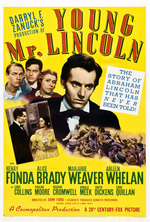
\includegraphics{Lincoln_tiny.jpg}
	\newpage

	\section{Racism - A most dangerous idea or concept - \textbf{18.11.2021}}
	\subsection{Definitions}
	\begin{itemize}
		\item{Race: "Race is humanity's most dangerous myth." as a social construct of beliefs and culture used to degregate people based on beliefs. "Race" as a term originated in the early modernity (16th century). Racialised societies created a hierachy. One example is the Chinese exclusion act in the US. But even before race existed as a concept, other things were used to define people, like:
		\begin{itemize}
			\item{Origin}
			\item{Gender}
			\item{Religious Affiliation}
			\item{Language: The Romans called people who did not speak Latin Barbarians}
		\end{itemize}}
		\item{Chattel Slavery: Cultural economic practices that tried to turn humans into a commodity. Garrison Frazier defined it as "receiving by the irresistible power the work of another man, and not by his consent" }
		\item{Slave trade: A large world system which linked Africa, Europe and the Americas through the slave trade triangle.}
	\end{itemize}
	About 10 to 15 million Africans were forcibly moved to the Americas. Around 15\% of them died during the voyage through \textbf{the Middle Passage}. After some time it was noticed that shark migrational patterns changed according to the slave trade. People who died or were about to die were thrown overboard and the sharks changed their behaviour accordingly. \\
	After some time slave holders realised that "if they were to keep the slaves healthy enough to bear more children than died, they could have a bountiful harvest of human capital" which only slightly increased living standards. \\
	The enticement of African tribes to capture and enslave enemy tribes to sell them, damaged the social structures of Africa to this day. \\
	On a slave ship, the average person had 4 ft\textsuperscript{2} of space. The system was designed to put people to a "social death" so they internalise themselves being property. \\
	\subsection{Slavery in the British Colonies - Involvement of the North}
	Teh entire American economy benefited from slavery. "Racial others" were used to define the dominant group. While it used to be based on religion, Catholicism and Protestantism, this was superceded by race. \\
	Slaves were used to grow rice or cotton, which were very labour intensive crops. 3/4 of the entire American cotton production came out of the American South. \\
	Nothern money financed plantations in the south. Northern insurance brokers helped finance them. Slave insurance were very popular and profitable as slaves were extremely valuable property and their loss meant serious economic damage for the plantation owner. \\
	A common economic cycle was the export of cotton produced in the south into the north, where it was turned into fabric and ultimately clothes, which were sold back to the south, to dress the peopl in the plantation. \\
	By the 1860s there were approxiamtely 4 Million slaves in the south. About one third of the population consisted of slaves. \\
	The value of slaves is underlined by the fact that plantations with more than 300 slaves were an exception. The majority of slave owners owned an average of 5 slaves. A lot of people in the south did not have slaves solely because they could not afford them, yet still benefitted from the institution of slavery. \\
	In the north slave owners were likened to "gracious care takers" of slaves to justify the continuous existence of this system. Even in the south the common opinion was that, "They may be holdin slaves, but at least they are taking good care of them". The bible was also used to a large extent to justify it. (Throwback to the "chosen people" of which the slaves were obviously not part of) \\
	\subsubsection{Dehumanisation of slaves}
	Slavery did not only deprive the slaves of social agency, they were also systematically robbed of their worth. Skin lighteners were very popular, even in the 18th century, to get a lighter skin. \\
	Slave owners used breaking up family dynamics as a demonstration of power and to instill fear. A family's child would be sold to another plantation owner to show that they could be sold and never be seen again at a moment's notice. \\
	Religion was introduced to slaves as a further means to "show them their place" as the stories were meant to reinforce their inferiority. Despite this initial motive, these same stories were used as a medium of hope, with, for example, Moses, who leads the oppressed people to safety, instead being used as a story of gaining freedom. \\
	In general there was always resistance, with the underground railroad only being one example of a very successful mode of liberation. \\
	\subsubsection{Whiteness crisis}
	As of 2020, the majority of 18 year olds, were no longer non-hispanic whites. \\
	Certain projections talk about in 2050 only 40\% of the population of the USA being white. \\
	The quote "Uneasy lies the head that wears the crown" talks about being dominant constantly puts you at risk of being toppled. While in the south only 1/3 of the population were slaves, there were areas where slaves outnumbered free people 1 to 10. If you are this outnumbered you are in constant peril effectively as an uprising can cost you your life. \\
	\subsection{The Abolition Movement}
	In the late 19th century several people felt like they should do away with slavery. Some abolitionists intended to relocate slaves back to Africa and bought huge swathes of land in Africa to relocate them. The country of Sierra Leone owes its existence to that. But while some took them up on the offer, many saw themselves as part of the American fabric. One person was \textbf{Frederick Douglass} who became one of the most outspoken Abolitionists and was also at one point the advisor to Abraham Lincoln. \\
	At the same time the Fourth of July was put into question. Frederick Douglass, talked about the Independence of the USA being an occasion for celebration only for free people, but for him it is a day of mourning. \\
	Another Abolitionist was \textbf{Harriet Beecher Stowe} who wrote one of the most well-known popular books about anti-slavery. \\
	\subsection{Slavery Compromises}
	The continued existence of slavery within the US was built on compromises. "The child of the west will unite the two warring parents [of slavery and free states]". \\
	One of the first compromises was the \textbf{Missouri Compromise}. Missouri was admitted to the union but already had a sizeable slave population, which was why they were allowed to be a slave state, despite being north of the 36th parallel. To bring parity in the states, Maine was formed. \\
	Another part of the compromise were much stricter slavery laws. Any person in a free state could, as long as one person states that they were a slave, be sent south. \\
	In addition all the "new states" in the west could decide by popular vote whether slavery would be legal or not. \\
	This led to pro and anti slavery supporters flocking to these states to influence the vote. At one point Kansas had two capitals, one pro and one anti slavery. \\
	\section{Civil War}
	In general the south had the upper hand with better leaders as well as a larger military. At first the north did not expect the south to really commit to this war. Only after some time did they realise that they had to invest massively into the war in order to be victorious. To this day the Civil War is the war with the most American casualties. More than any other hostile conflict combined. \\
	\subsection{The Gettysburg Addres (19.11.1863)}
	On that day the president delivered the "Gettysburg Addres" talking about what being in the nation means. Previously talked about topics of what makes an American are addressed. To this day people in the United States of America on a high school level learn this addres by heart and recite it publicly. Things like the Puritan Jeremiad are referenced. The Civil War is framed as a second Revolution. A battle in which the ideals are fortified, or shattered. But he also talks about hope for the future, to be redeemed and to live up to the lofty ideals and that in the future more people would be included in the "we, the people" \\
	American Exceptionalism at work here, once again, is stating, that "if we fail, how can anybody else succeed?". \\
	\subsection{Reconstruction}
	Even before the war was won, there were promises made for the future. These were:
	\begin{itemize}
		\item{Emancipation of slaves}
		\item{Occupation and sharecropping}
		\item{Amendments passed to free black people}
		\item{Jim Crow laws}
	\end{itemize}
	\subsubsection{Occupation}
	The period of time after the war was Reconstruction, which was a reconstitution of the US. The southern states were in military occupation for 7 years, they were forced to abolish slavery at gun point. \\
	Right after the war black universities were founded in troves to educate these newly freed people. \\
	\subsubsection{Sharecropping}
	While it was at first promised that the land would be given to the freed slaves, this did not come to pass. Instead a system called sharecropping started, where people would work on the same field but get a share of the crops they farmed and in turn would be cared for with housing or food. This is usually seen as little more than rebranding as, while it was not slavery anymore, there was still dependance. \\
	\subsubsection{Amendments}
	In the 13th Amendment slavery was outlawed, even before the war was won. \\
	In the 14th Amendment it was made illegal to discriminate based on race in court. \\
	In the 15th Amendment all black males were given the right to vote, thus making not letting people vote against the constitution. \\
	\subsubsection{Jim Crow laws}
	But states could still require people to prove that their fathers were already allowed to vote, restricting some people again. There were also literacy tests tied to the right to vote, which many blacks could not pass. \\
	This meant that the Reconstruction, introduced with lofty goals, petered out over time. \\
	In the south a system of segregation was established. Jim Crow laws were enacted that seperated whites and people of colour in a "separate but equal" society. This still boiled down to a "separate but unequal" as, for example, schools were generally segregated but had white schools well funded while black schools being in squallor. \\
	\subsection{Slavery today}
	Even today 20 million people find themselves in a form of unfree labour. Places like Dubai still employ a form of sponsorship to bring foreign workers into the country but requiring them to give up their passports and forcing them into near slavery under the threat of deportation. \\
	\newpage
	\section{Week 7: Westward expansion - 25.11.2021}

	One of the biggest myths about the west is that it was empty before the westward expansion happened. When Spanish came from Mexico they considered it the north, the French headed south and the Chinese came from the east but only when the Americans appeared did they coin the term "The West". But to the people who had lived there for centuries, they considered it home. \\
	The term "West" is only very loosely defined. They asked experts on the West three questions:
	\begin{itemize}
		\item{Where does the West begin?}
		\item{When did the West begin?}
		\item{What are striking features of the West, separating it from e.g. the Midwest?}
	\end{itemize}
	Most people, after having been asked the first question pointed westards as "somewhere out there" and depending on where people considered it differed greatly. People in Canada considered different parts of the West than Americans did. Many people also equated the West with the historical frontier On the other hand it was relatively clear where the East starts, which was between the 100th and 98th Meridian. There, the Great Plains start and there is less rain than in the east. This line of aridity is called the "isohyetal line" and it is said that "water deficiency is one of the most defining features" of the area. \\ \\
	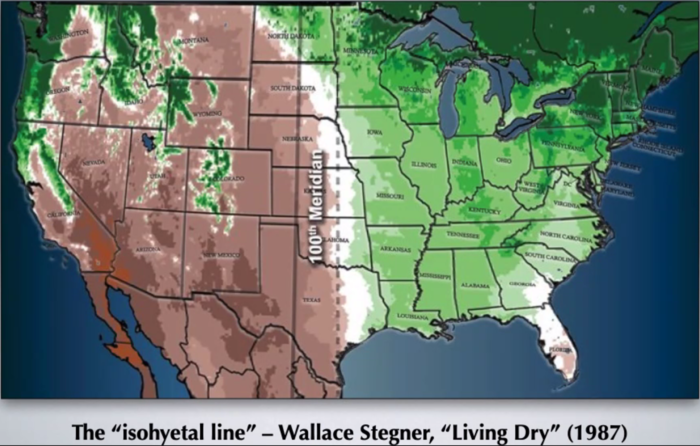
\includegraphics{isoyhetal_line.png} \\
	But there is also a continuous debate between old and new historians. There is a lingering influence by the so called "Turner School" who defined the west as a process or progress, which makes the West less of a place but more of an outcome and state of mind. \\
	In an nutshell (Yet these are not definitive answers or definitions) the west can be understood as a triangle between History, Geography and Imgaination. That, when you talk about the West you talk about the historical West, the geographic West and the psychological West at the same time. \\
	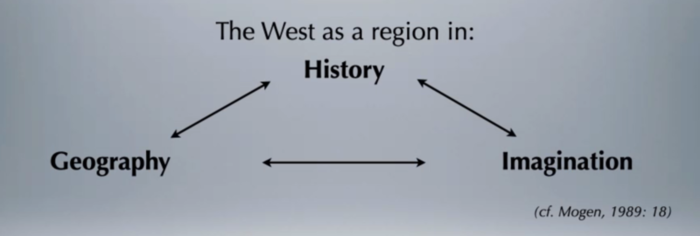
\includegraphics{Understanding.png} \\
	During the colonial era both African and Indigenous people were considered "lower" in the evolutional ladder (Which was one dimensional) and that by "showing" indigenous americans the way they could catch up. On the other hand African people were not considered capable of progress at all, being similar to apes and never able to catch up. \\
	\subsubsection{Northwest Ordnance}
	With the Northwest Ordnance an act was established to handle introduction of territory and how to handle native americans. A new territory could be integrated into the union the moment it had 60,000 inhabitants. It was also established that native americans had a right to their land but which had to be claimed. It acknowledged that they were independent people and had to be treated as officials from other countries. This influences legal battles even today as most promises that were made over the centuries were broken at some point. Fortunately these were all documented so native american tribes are aiming to reclaim their rights even today. \\
	\subsubsection{Louisiana}
	In 1803 Thomas Jefferson negotiated a real estate deal with Napoleon, as they needed money, and acquired the state of Louisiana, doubling the total area of the USA over night. An expedition was sent, called the \textbf{Lewis and Clark Expedition} They were sent to search for a waterway to navigate the country easily. While this was not found, there was another objective to this expedition. As there were a lot of myths, for example one that dragons roamed these lands, they were tasked to make notes of every animal and plant they saw. \\
	Jefferson expected Americans to require 10 generations to "fil the canvas". This also included native americans, who were expected to give up their ways and become farmers. \\
	At the same time people in the area of \textbf{Mexican Texas} started revolting against the Mexican government in the \textbf{Texas Revolution} of 1835 and gained independence 1 year later. This Republic of Texas lasted for 10 years until American troops annexed the territory and incorporated it into the USA. At the same time thirt-two American Immigrants staged a revolt agains the Mexican government and locally raised the flag of a new breakaway republic. This only lasted for 25 days when a battaillon of American troops raised their flag in the state. This started the \textbf{Mexican-American War} which saw the territories of California, Texas and New Mexico ceded to the US. \\
	Also at that time did James W. Marshall find gold at a place called Stutter's Mill. These news spread all over the country and over the next 8 years 300,000 people travelled to California to find gold themselves. In 1849 alone 60,000 people arrived in California.
	By the middle of the 19th century America had established itself across the continent.

	\subsection{Manifest Destiny}
	Americans at that time (and to a certain extent still today) considered themselves culturally and evolutionary superior and it is their destiny to spread their way of life and governance. American democracy and government were interwoven with this, where the "wild lands" of the west were to be made cultured. At the same time Americans did not consider themselves as similar to the "Old World". \\
	One of the most well known pictures exemplifying this is called "American Progress" by John Gast. You see "Columbia" going westwards, in this case Texas, a school book and landline in hand to bring civilisation to the wild lands. The west is dark and the east is lit up, and wherever the Americans go light and progress come as well. Pioneers and gold miners come to seek out riches. Later settlers appear to till the land and in the back you can see civilisation appearing in the eastern background. This is not the only painting of this kind, in fact there was a whole family of paintings being created at that time. \\
	But as opposed to what is being shown in this painting, at no point was this "progress" as linear as portrayed. \\
	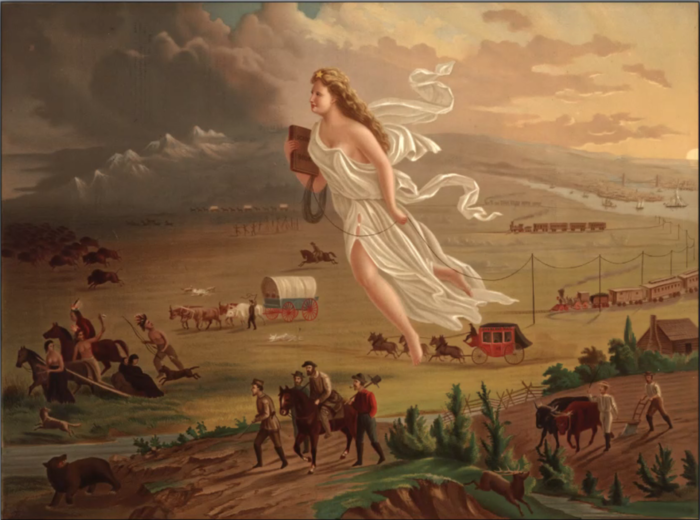
\includegraphics{American_Progress.png} \\
	\subsection{The Indian Problem}
	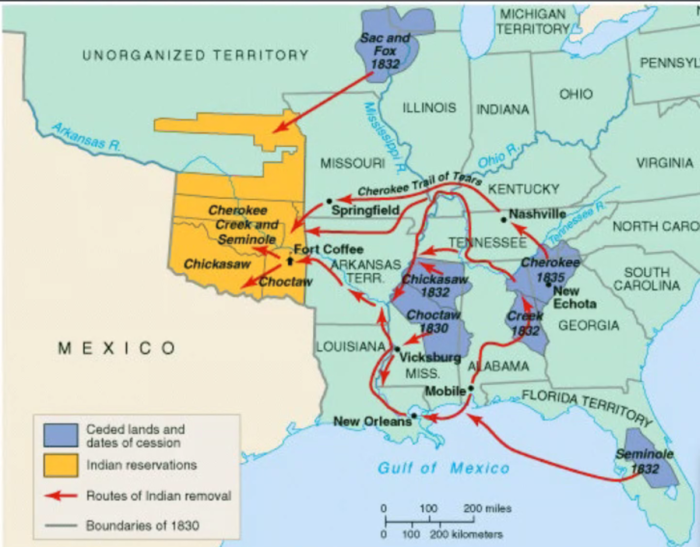
\includegraphics{Trail_of_Tears.png} \\
	Over time close to Arkansas there was a greater need for farm land and living space. Some tribes tried to assimilate to the Amercians. These \textbf{5 civilised tribes}, the Cherokee, Creek, Seminole, Chickasaw and Choctaw developed a written language, a constitution and much more in order to show that they would like to be part of the US. A plan of the US was to create a reservation close to Arkansas west of the Mississippi River as these lands were generally seen as untillable and only good for savages. To get them there these civilised tribes were put into concentration camps and then herded to the reservation. This is today known as the \textbf{Trail of Tears}. Before this happened the tribes actually tried to sue the government and the courts ruled in their favour but president Andrew Jackson chose to just ignore the verdict and did it anyway. \\
	While at first there was a plan to establish a permanent reservation in the heart of the country, this was soon abandoned as the need of land rose. \\
	\subsubsection{Native resistance}
	Over time bloody conflicts ensued between the US and native americans. Native Americans tried to resist and also had two major victories, especially the one won by the tribe chiefs \textbf{Sitting Bull and Red Cloud} at the \textbf{Battle of Little bighorn} where one battaillon of military forces was wiped out. Another one was \textbf{Geronimo} further in the East where the military was resisted for several years.
	While there were victories, native americans were ultimately beaten resoundingly as it resulted in a major war of attrition. At the same time the fauna of the plains was decimated. While at some point there were estimated to be 50 million wild bisons the Smithsonian Institute had major problems finding 25 specimen to observe. \\
	Afterwards the treaty system that forced the US to treat native americans as foreign nations was abolished (But later reintroduced and kept up to this day) which made the requirement to make treaties with tribes not necessary anymore. \\
	With this a cultural genocide happened. Native american children were put into boarding schools to "condition them to become good americans". This included forcing them to wear western clothes, not allowing them to perform their own rites or practice their own religion. If they were caught speaking their own language their mouths were washed with soap. While boarding schools were only short-lived it still had a disastrous effect as around two generations of native american children were completely detached from their native tribe often not being able to speak the language. It also did not have the desired effect as these forced measures did not lead to them becoming "productive members of society". \\
	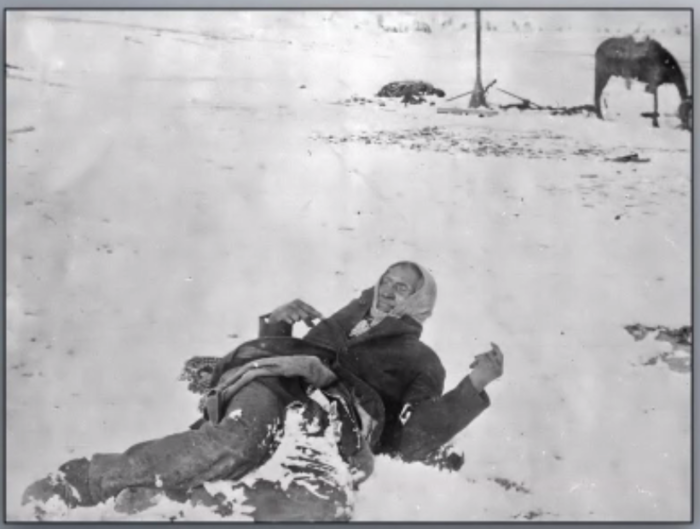
\includegraphics{Wounded_Knee.png} \\
	The last major form of resistance was broken at the \textbf{Massacre of Wounded Knee}. American soldiers claimed they were being attacked even though it was later proven that they were only trying to move camp. The main motivation for this massacre was retribution as a lot of the soldiers who committed this were part of the battle of little bighorn. \\
	Today native americans in reservations have some of the highest cases of alcoholism and drug abuse in general. Young native americans show some of the highest rates of suicide and many who leave the territory become increasingly disconnected from their tribe, showing that the actions from 150 years ago still have an effect today. \\
	\subsubsection{Closing the Frontier}
	After the Massacre of Wounded Knee the frontier was considered to be closed but since the frontier had been one of the main points of American development. To comment on this \textbf{Frederick Jackson Turner} he penned a paper and showed it at the World's Columbian Exposition 1893. He spoke about general anxiety about the frontier being crucial to the american idea. He said that "The existence of free land and continuous expansion explain American development" and that closing the frontier closed the first chapter of american history. This continuous expansion made America, according to him, exceptional. But since the frontier was now about to close, how could they continue to be great? Thus did they start to expand beyond main land America and conquered their first overseas territories, establishing themselves as a global player. \\

	\section{Week 8 - The mythic west and popular culture - 02.12.2021}

	Usually the West, mostly in Western movies, cowboys are white men, with bandits or native americans as the antagonists in the story. Despite this, it is estimated that between one third and half of all cowboys has African American roots. \\
	The West is the "longest running drama in American popular culture". The mythic West features readily recognisable heroes and well established tropes. It established white Anglo-Saxon Protestant as the norm in that area. \\
	\subsection{Pre-19th century roots}
	Early colonial writing blends facts and fiction in addition to sensationalism and religious doctrine. The most popular subjects was the New World flora fauna where fantastic stories about giant wild horses that were so tall that they had to sleep leaning on a tree. Rattlesnakes were also of particular interest where they could bite chunks out of people and hypnotise them. \\
	The second one were the New Worlds inhabitants. The division between noble and ingoble savages stems from this pattern. It is likened to Adam and Eve with the nobel savage being very open to the "new" and "better" old world. \\
	Then there is also the ignoble savage who is a barely human heathen, drinking in abundance and, most of all, resistant to the progress brought by the settlers. \\
	Another genre is the capvitiy narrative, particularly the \textbf{Captivity of Mary Rowlandson} written in 1682. It was at that time very common for Native Americans to take captives in order to bolster their losses as well as weakening the enemy by stealing children and women. In Mary Rowlandsons captivity she uses religion which let her "keep her culturedness" despite the influence from the native americans and ultimately able to escape and have her restored. This sparked a whole genre and spawned several hundreds of captivity narrative stories. This can be likened to J.K. Rowling or Stephanie Meyer who started their own genres (Of questionable content). \\
	Even today these saviour stories, like Avatar (2009), still exist where a white man is exposed to a native culture, be it Native Americans, Asians or even foreign planet's societies, and after having met them fights his old colonisers in order to protect the native population. This is a very American formula
	\subsubsection{American Romanticism}
	In American Romanticism, the elements of this mythos that has already been established, and provides a template for a geneology of heroes that still exists today. Outlaws, heroes and even anti-heroes are part of the archetype established at that point. \\
	\subsubsection{Dime Novels}
	One standardisation of this mythos als owas the \textbf{Dime Novel} that appeared in the 1830s to great popularity. This was due to an explosion of the home market, with levels of literacy increasing, which made people want to read. This was also helped by the fact that they were very cheap, where you'd get one dollar worth of book for only one dime. While it was, at first, only a niche, it eventually mushroomed to a much larger genre. In the UK these were called \textbf{Penny Dreadfuls}. They were always small booklets that were easy to make and easily portable. The books were always very melodramatic, taking established characters and making them over-the-top. The general plot were white men saving white women by killing indiands. This created stock characters that could later be ported to different genres. These books can be compared to modern super hero movies, which have at this point also become very formulaic and standardised. \\
	One popular figure was \textbf{Kit Carson} who was a famous  cowboy. People who had never been to the West save met Kit Carson, wrote Dime Novels about his adventures to the point where people who met him were convinced it wasn't actually him because it didn't line up with his persona in the books. \\
	This also created the \textbf{Social Bandit or America's Robin Hood} who were "good" bandits and talked about class conflicts in the west. Together with othe forms of media at that time this created the \textbf{Lone Ranger} archetype. \\
	\subsubsection{Wild West Shows - Buffalo Bill}
	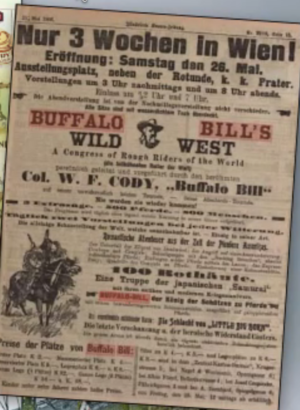
\includegraphics{Buffalo_Bill.png} \\
	After the end of the advancement of the frontier that led to a sort of loss of purpose, William F. Cody, better known as \textbf{Buffalo Bill} created a Wild West Show to reenact bison wrangling, texas shootouts and other things. He was so popular that most bigger monarchs in Europe came to watch him. He even stayed in Vienna for 3 weeks, performing for the Monarch as well as anybody who could afford it. \\
	These wild west shows are considered institutionalised ceremonies. Due to an impending sense of loss of the identity of the West after immigration from other parts of the world, these shows showed what people wanted to see in the West. They showed the things that people wanted to see. The shows relied heavily on real Native American people, where he, for example, hired \textbf{Sitting Bull} for his shows, who also recruited other people from the plains tribes. This was rather damaging to the perception of Native Americans as because of that all native people of North America were seen as plains tribes, with tipis and feather headdresses hunting bufallos, which in no way all native american people did. One deconstruction of this stereotype existing until today is the movie \textbf{Smoke Screen} where there is a scene about native americans having to be stoic and acting as if they "just came back from buffalo hunting" to which one of the characters responds that his tribe were fishermen and never hunted buffalos. \\
	\subsection{The Golden Age of the Western (as a genre)}
	With the novel \textbf{The Virginian} by Owen Wister the Western reached a point of Genesis with a nameless cowboy hero who is inbetween worlds. There is also corrupt institution with a big landowner being the antagonist of the western rancher with a final shootout at the only time where shootouts can happen, after which he rides into the sunset. This formula was extremely persistent. When the West stopped being a factual thing, the mythological west came into existence, that existed independent of time, never changing. The formula introduced by The Virginian continues in movies and television shows today. It also exhibits a very clear line of morality, with clear segregation of good vs. bad and the outcome that all bad men deserve to get shot. \\
	In 1903 another milestone was reached with \textbf{The Great Train Robbery} becoming the first Western movie. It showed all of the archetypes you would expect from a western with the robbers having a shootout after which the hero rides into the sunset. \\
	\subsection{Decline of the Western}
	In the 60s four big things happenes which had an influence on the decline of the Western:
	\begin{itemize}
		\item{Vietnam}
		\item{Civil Rights Movements}
		\item{Sexual Revolution and Women's Rights movements}
		\item{American Indian Movement}
	\end{itemize}
	These civil rights movements combined made the Western the way it had been a bit problematic because the mythos up until that point had been primarily of Anglo-Saxon white men. \\
	In addition many of the people who went to fight in Vietnam grew up on Westerns and they saw themselves as heroes swooping in on the Communists and routing out the Viet Cong. This was in stark contrast to the actual experiences there, where many experienced gruesome mutilations and atrocities which was in satrk contrast to their jongistic ideals. \\
	This gave way to \textbf{Revisionist Westerns}, which rose in popularity as the old westerns declined. One of the first forms of Revisionist Westerns were Italian and Spanish \textbf{Spaghetti Westerns}. In these Westerns the hero fights viciously, but not for moral reasons. There is also no transformation of the hero throughout the movie. \\
	While we enter the present day of Westerns, these clear cut categories of Westerns are muddied with some movies having Western as well as Revisionist Western characteristics despite not being Western type movies. The movie \textbf{Dances with Wolves} was, at the time of release, lauded as a "new type of Western" despite, in retrospect, still exhibiting many of the stereotypes of Westerns with a white hero escaping civlisation and the Native American people being patronised to a certain extent. \\
	There is today an ongoing renaissance of Western movies with a resurgence of Western tropes appearing again though not necessarily in Western movies. \\

	\section{Week 9 - Addressing the "unfinished business" - 09.12.2021}

	The Term \textbf{The American Century} was coined by Henry Luce shortly before they joined the second World War saying that: "We must undertake now to be the good Samaritan of the world", which again ties into the Puritan origins and American Exceptionalism. \\
	The American Century can roughly be divided into three eras as well as two crises, which were followed by great change:
	\begin{itemize}
		\item{The increase in affluence in the 1920s (The Roaring Twenties) as well as the following stock market crash and Great Depression.}
		\item{Following the second World War saw the US as the most powerful country, but also put it under a lot of international cultural strain. A consequence of this was a resurgence in Conservatism, which, among other things, saw the election of Ronald Reagan}
	\end{itemize}
	\subsection{Struggle for social justice}
	During World War I and World War II there was a particular belief that, if they go to fight for their country they will ultimately gain the respect of their countrymen and "prove their worth". \\
	A particular black man, who lived in France when WWI broke out joined the French infantry, was wounded and was awarded one of the highest honours after he recuperated. He then joined the French Air Force but later wanted to join the American Air Force instead, where he was rejected as, at that time they only accepted white pilots. After the war he returned to the US. When a French president visited the US he wanted to meet him as he was considered a war hero of France. After they spent considerable effort finding him, it turned out that he was working as an elevator operator, barely making ends meet as he was completely unknown in America. \\
	\subsection{Early 20th century status quo}
	After slavery was abolished a "Separate but equal" system was established, which meant de jure segregation in the south and de factor segregation in the north. At this time the district of Harlem in New York became the centre of black culture with the \textbf{Harlem Resistance} forming. \\
	In World War II more than one million black men joined the military to fight for their country. At this time the military was strictly segregated with no mixture between races happening in platoons. There even was a blood bank for black and white soldiers in order for no white soldier to receive a black soldier's blood. \\
	At the same time Asian internment camps on US soil were established. Over time more than 100.000 Americans of Asian descent were interred in, not death camps, but little better than that, concentration camps. \\
	\subsubsection{Civil Rights watershed events}
	During the 50s there were several milestone events that aided the right
	In 1896 a Supreme Court Ruling, which stated that segregation was permitted, if both facilities are of equal quality, which was never the case. This ruling was, little by little, dismantled by proving that the facilities were not of equal quality. \\
	In 1957 black students at Little Rock Nine High School were escorted by 1000 soldiers for one year in order to go to a white high school as they were harrassed on their way to school. \\
	Another event was Rosa Parks in 1955, where Rosa Parks, a black woman, refused to go to the back of the bus when a white person wanted here seat. She was arrested, as it was the law, but a boycot by the black community made the bus company get rid of this law. \\
	In 1960 Sit-In Movements in many diners were
	These cases were not only an issue nationally but also internationally, as the perception of US-Americans at that time, was that they were the paragon of virtue and democracy. How could they claim to be that if they denied these rights to some of their own citizens? \\
	\subsubsection{Martin Luther King}
	When Martin Luther King (MLK) started his movement, he initiated non-violent protests, where protesters were dispersed with water cannons without resisting, showing these pictures of brutality in the world. Later he gave his most popular speech "I have a Dream" using the very same rhetoric that the dominant culture in the US had been using for centuries. \\
	In his speech in 1963 he talks about having entered a social contract through the \textbf{Emancipation Act}, signed by Abraham Lincoln "5 score years ago". But despite this promise black people are still segregated in their own land, which is why he had come on that day to cash in that promissory note about being guaranteed the unalienable right of liberty and pursuit and happiness. He claims the US having defaulted on this promissory note, which is why black people were given a bad cheque. But since he refuses to believe that the "Bank of Justice" is bankrupt, he has come today to cash in on that cheque. \\
	He used the term "promissory note" as this was the same concept used by the Founding Fathers. According to him, black people, until this point still had yet to cash in on this cheque. He also uses the Puritan Jeremiad as a rhetoric device, by talking about the current hardships, while highlighting the golden era of the past to ultimately state hope for the future. Not a distant future but a future that is now, while also warning his brethren to not lash out in violence as people belong together. \\
	While this was just a speech, it has lasting political effects. President Kennedy, while at first hesitant, vowed to address these injustices. Even thoug he did not manage to do that, as he was first assassinated, his Vice President enacted the \textbf{Civil Rights Act} of 1964 ending segregation as well as the \textbf{Voting Rights Act} in 1965. \\
	\subsubsection{Malcolm X}
	At the same time \textbf{Malcolm X} also became more known. In opposition to Martin Luther King, he sought for Black Separatism, rejecting the basic American social contract, as it was, in his eyes, only for white people. He was assassinated, even before Martin Luther King, and was not able to see his plan come to fruition. \\
	\subsection{Post-Racial Society?}
	Over time more legislation was passed for social justice, with affirmative action being enacted as well as more equal employment opportunities up until the first black president was elected with \textbf{Barrack Obama}. This purpoted post-racial society in the US, was only an illusion though. Despite there having been a black president, black people within the US still experience far higher incarceration sentence, which is commonly called the "school-to-prison pipeline", where black people often go directly from high school to prison, where they can legally be used for cheap labour and denied the right to vote. \\
	Acording to latest census data, almost one third live below the poverty line. Black men are six times more likely being incarcerated than white men. There have in recent years been ugly landmarks of incidents, showing that racial tensions still exist to this day. \\
	\subsection{Indigenous survivance and resistance}
	Following the Wounded Knee Massacre had their population dwindle to less than 250.000 people. Only in 1924 were Native Americans granted full citizenship with the \textbf{Indian New Deal} as well as giving them back their sovereignty. Over time there were several pushes to assimilate Native Americans, in line with "Kill the Indian, save the man" but in the 1960s there were pushbacks to this policy and aims to gain the right to self-governance. In 1969 Native Americans occupied Alcatraz, which had fallen into disrepair, in a symbolic act of reclaiming land. In 1968 they were granted semi-sovereignty within the United States as well as the right to self-government. There were also lawsuits for restitutions, which are ongoin to this day. But over time these movements have been marred by inter-tribal corruption in Native American communities. \\
	\subsubsection{Native American Renaissance}
	Native American literature received international recognition with N. Scott Momaday winning the Pulitzer Prize in 1969 with his book titled \textbf{House Made of Dawn}. From this moment onward Native American literature had a surge in popularity and output of Native American literature. \\
	One of the central themes in his books was finding a sense of self for Native Americans, as life in urban areas usually meant poverty. He also talks about returning Native Americans veterans, as they, just like black people, had a disproportionally high percentage of people who served in the military. \\
	\subsubsection{Concerns in "Indian Country"}
	Within Indian Reservations there still are significant health disparities, with COVID having hit them much more significantly. In addition to general disparities based on health care, they also face threats to indigenous sovereignty, with mining or logging companies infringing on their territory. \\
	
	\newpage
	\section{Week 10 - American Imperialism abroad - 16.12.2021}
	
	When the US closed the frontier at the beginning of the 20th century, there were questions about what to do next, as the mythos of 'progression' had been a cornerstone for American self-image. \\
	At this time the general consensus within the US was, that they did not want anything to do with imperialism. This was mainly because they compared themselves to European empires like the UK and Spain, and did not want to be 'just another imperial power'. Many scholars like Carnegie argued that the way the European powers did imperialism, is actually anit-American. \\
	While there was anti-imperailist sentiment, the frontier and 'going westward' was just another form of imperialism. This left them with two options: Either not starting European type imperialism or inventing 'their own' kind of imperialism. \\
	The latter happened as Cuba rebelled against the Spanish empire and America dispatched troops to 'aid' them. After only 4 months they had acquired a new possession for themselves. The same happened in Hawaii, where business interests led to a coup. After this had happened very few argued for returning these newly acquired possessions. \\
	\subsection{America in World War 1}
	When America entered World War 1, they only participated for a very short time, 19 months in total. In fact, more soldiers died from diseases, than were killed in battle. \\
	When the Treaty of Versailles was drafted, President Woodrow Wilson, who was the first president to travel abroad, revealed his \textbf{Fourteen Points}, which was an outline of imperialist structures. \\
	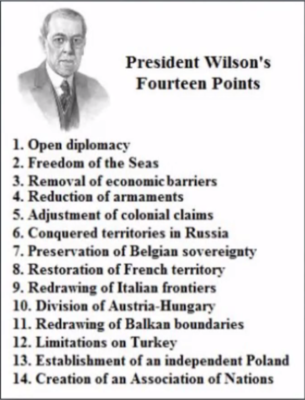
\includegraphics{Fourteen_Points.png} \\
	Ultimately his fourteen points failed, as most parties in it were mainly interested in punishing Germany, while also sharing the spoils of war among themselves. While it failed, the founding of the \textbf{League of Nations} ended up actually happening. Despite the US having proposed it, they ultimately did not join as the Senate blocked it until it disbanded. \\
	The end of World War 1 'supercharged' the American economy as they were not ravaged by war and could sell their goods to the rest of the world. This also led to Wall Street becoming the financial capital of the world, taking it from London. During this time the US-Dollar also established itself as the de facto currency and American society started becoming a 'credit society'. \\
	At the same time Hollywood became an important centre of entertainment, moving away from New York, after movie industries in Europe were destroyed, with France having been the biggest producer of movies before. \\
	\subsection{Cold War}
	After the second World War, the US was very interested in forming Europe and also Asia into a free-market society, as this was good for business, where they can export their own goods. At the same time the USSR was concerned with Germany becoming a powerful nation again, which is why they 'encouraged' Eastern European countries to adopt socialist governments as a buffer to Germany. This saw the US entering a policy of \textbf{Containment}, to decrease the influence of Communism. At this time Communism was turned into a boogey-man, which has to be stopped at any cost. \\
	This saw the introduction of the \textbf{Marshall Plan}, which tried to finance the rebuilding process of Western Europe, which was supposed to not only create a continent of consumers of American goods but also stop Communism from spreading. \\
	When \textbf{John F. Kennedy} gave a speech about the 'New Frontier', where he alludes to old deals, made by former presidents like Woodrow Wilson, and also, as always, using the Puritan Jeremiad, in his speech. With his New Frontier, he aimed to officially accept the 'role of the leader of the free world'. \\
	At this time the US-American GNP made up almost 50\% of the world's total. This decreased to 25\% until the 1970s, when Asian and European countries had rebuilt somewhat. This figure has since stayed stable, and will likely stay that way for at least a short period of time, when China emerges even further. \\
	This marked the start of American 'soft power' imperialism, through their products. Two very obvious examples of that are:
	\begin{itemize}
		\item{During the Cold War American soldiers stationed throughout Europe actively encouraged the consumption of American media. There have also been \textbf{America Houses}, officially meant to promote de-Nazification, while also spreading American culture. They had an open library, where people could borrow American books, as well as offering English courses and holding American centered cultural events like concerts and readings. These houses were established all throughout Europe, from Norway to Italy, also using them as launching pads to spread American culture throughout Europe by, for example, library buses.}
		\item{Something called 'Coca-Cola Colonialism', later replaced by 'McDonaldisation', where American cultural companies like McDonalds and Coca-Cola spread throughout the world. Since these companies also bring American cultural values, this can lead to homogenisation as it replaces the unique culture of that area with the standardised items of the companies. Major tenets of this process are:
		\begin{itemize}
			\item{\textbf{Efficiency:} The optimal method of acomplishing a task. With Mcdonalds it is the fastest way of getting from being hungry to being full. Everything is geared towards efficiency.}
			\item{\textbf{Calculability:} Having quantifiable objectives. Instead of trying to deliver the best product (With taste being a very subjective and not quantifiable thing) to only focusing on sales. This means that instead of trying to deliver quality, trying to deliver as many products as possible. This has also led to the assumption that large sales equals good quality; The best product sells the most, which isn't necessarily the case.}
		 	\item{\textbf{Predictability:} Standardised and uniform services. Delivering the same product everywhere, means that people can know what to expect no matter where they are. This is the same with the employees in such places, having highly repetitive and predictable tasks.}
		 	\item{\textbf{Control:} Controlling every aspect of one's sale. Employees wear the same outfit, use the same greeting etc. This is achieved even better by machines, who by design always do a task the same way.}
		 \end{itemize}}	
		 This also extends to entertainment. Movies coming out of Hollywood are extremely formulaic, so they appeal to as large of an audience as possible.
	\end{itemize}
	At the end of the Cold War, when the USSR collapsed, the US was left standing as the sole super power. This just confirmed the views many Americans had held all this time, of them being the world leader and the chosen people. In movies like \textit{Indpendence Day} or \textit{Armageddon}, it is always the American president holding a speech, observed by the whole world, in order to avert a disaster that threatens the whole world. And it is always a group of all American heroes rising up to the task to save everybody. \\
	While during these times the US saw itself as the leader of the world, the question goes back to Crevec\oe 'What this new man called American' is. The dominant theory in America is the 'melting pot', where all of these cultures are put into one big pot and then homogenised in an effort of assimilation. This was enforced by having people undergo through 'training' and only allowed to participate in the American culture when it has been achieved. \\
	Another theory, competing with the melting pot, called the 'Salad Bowl', intends to not assimilate cultures, instead promoting multiculturalism, where all of the cultures are in one big bowl, but all of the individual bits and pieces are still visible and discernible. \\

	\section{Week 11 - Revisiting the American Dream in the 2st Century and the myth of upward mobility - 13.1.2022}

	Andrew Carnegie, known as a philanthropist, having built public libraries throughout the US, was also a ruthless industrialist busting unions and squeezing labour out of his employees. He, among other people, is seen as an example of a product of the 'American Dream'. The story about working hard and thus making it big and getting rich in the US is a story that has existed for centuries and is seen as a core tenet of an American's self-image. \\
	The workings of this 'entrepeneurial spirit' has permeated large parts of society with kids already entering the 'hustle', selling lemonade or other things. \\
	But despite what some people might want you to think, entrepeneurship was not invented in America but originates from Anglo-Saxon settlers. \\
	\subsection{American Idealism}
	What is today known as American Idealism, which kind of resulted in the American Dream has its roots in the very first settlers who came to America, taking risks and taking the chance of failure, which was still better than the status quo of persecution in Europe. This is coupled by things like the prosperity gospel, that God loves you if you make it and get rich, originating in Puritanism. \\
	Even after the constitution was enacted, this kind of thought continued, declaring 'the pursuit of Happiness' as an unalienable right. This essentially formed a massive free-trade zone ensuring uniformity between trading partners within all of the United States. \\
	\subsection{Horatio Alger}
	It was Horatio Alger who became synonymous with 'Rags to Riches' stories. At that time there was a massive amount of homeless children in New York and when he saw a homeless boy one day, he thought about what he could do to help them as any of these children could become successful but also end up as thiefs or dead. This birthed his stories about homeless boys he met, creating characters like 'Ragged Dick', 'Pluck and Luck' and 'Tattered Tom', where they are at first betrayed by a trusted associate but then, through the guidance of a mentor make it in the end. These proved very popular and he used most of the money he made from it for philantropic purposes.

	

	
	
	































	
\end{document}